\documentclass[11pt]{article}

\usepackage{amsmath}    % need for subequations
\usepackage[utf8]{inputenc}
\usepackage{graphicx}   % need for figures
\usepackage{verbatim}   % useful for program listings
\usepackage{color}      % use if color is used in text
\usepackage{subfigure}  % use for side-by-side figures
\usepackage{hyperref}   % use for hypertext links, including those to external documents and URLs
\usepackage{afterpage}  % create blank page
\usepackage{appendix}   % create appendix
\usepackage[a4paper, margin=2cm]{geometry} % change margins
% \usepackage[french]{babel} % permet guillemets etc
\usepackage[british,UKenglish,USenglish,english,american]{babel}
\usepackage{wrapfig}
\usepackage{sectsty} % color title
\usepackage{eurosym}
\usepackage{tabularx}
\usepackage{anyfontsize}
\usepackage{tikz}
\usepackage{fancyhdr}
\usepackage{eso-pic}
\usepackage{minitoc}

%%%% Couleur des titres
\definecolor{green}{RGB}{134,188,37}
\definecolor{blue}{RGB}{98,181,229}
\definecolor{teal}{RGB}{0,151,169}

%%%% Themes
\fancypagestyle{theme}{
\fancyhf{}
\fancyhead[L]{}\fancyhead[C]{}\fancyhead[R]{\rightmark}
\fancyfoot[L]{Cassiopée 2018-2019}\fancyfoot[C]{\thepage}\fancyfoot[R]{}
\renewcommand*\headrulewidth{1pt}
\renewcommand{\footrulewidth}{1pt}
}

%%% Box
\newcommand{\titlebox}[2]{%
\tikzstyle{titlebox}=[rectangle,inner sep=10pt,inner ysep=10pt,draw]%
\tikzstyle{title}=[fill=white]%
%
\bigskip\noindent\begin{tikzpicture}
\node[titlebox] (box){%
    \begin{minipage}{0.94\textwidth}
#2
    \end{minipage}
};
%\draw (box.north west)--(box.north east);
\node[title] at (box.north) {#1};
\end{tikzpicture}\bigskip%
}

%% Custom packages
\usepackage{listings}

%%% Table
\usepackage{array,booktabs}
\usepackage{tabularx}
\usepackage{ragged2e}
\usepackage{hhline}
\newcolumntype{x}[1]
{>{\raggedright}p{#1}}
\newcolumntype{z}[1]
{>{\centering}p{#1}}
\newcommand{\tn}{\tabularnewline}
\renewcommand\tabularxcolumn[1]{>{\Centering}m{#1}}  

%%% Custom
\newcommand{\ptitle}[1]{\underline{\textsc{#1}} }
\newcommand{\Q}{\underline{\textsc{Question :}} }

\pagestyle{theme}

\thispagestyle{theme}

\newcolumntype{b}{X}
\newcolumntype{s}{>{\hsize=.5\hsize}X}
\usepackage{graphicx,lipsum}
\begin{document}

\begin{center}


\includegraphics[width=0.3\textwidth]{images/logo.png} \\ \vspace{0.4cm}
{\huge \textsc{Cassiopée Project 2018-2019: Development and deployment of an automated IT security audit tool in a virtualized environment.}} \\
  \textit{Aurélien Duboc, Pierrick Gorisse, Lucas Martin \\ Supervisor: Hervé Debar}

\end{center}

\noindent\rule{\textwidth}{.1pt}%
\tableofcontents
\noindent\rule{\textwidth}{.1pt}%

% \section{Cassiopée Project: Development and deployment of an automated IT security audit tool in a
% virtualized environment.}
\section{Start of the project}

\vspace{1cm}

Large companies as well as SMEs are subject to a security obligation
for their information systems. The idea is to propose a tool that allows the
management of the main vulnerabilities that security auditers usually look for.
This tool will identify several weaknesses and / or configuration vulnerabilities.
\\
The main interest lies in the automated analysis of a large number of machines. 
It could also propose automated corrections associated with these weaknesses. 
One could imagine that a tool like this one, to which other features would be 
added, could be a security audit equivalency for companies 
if this tool is accredited.
\pagebreak

%% List of tools, useless according to Hervé Debar

%\subsection{Technical ressources}
%
%\begin{tabularx}{\textwidth}{bs}
%  \hline
%    \begin{flushleft}
%    (1): Proxmox VE is a complete open-source platform for enterprise
%    virtualization. With the built-in web interface you can easily manage
%    VMs and containers, software-defined storage and networking,
%    high-availability clustering, and multiple out-of-the-box tools on a
%    single solution.\\ *\url{https://www.proxmox.com/en/}
%    \end{flushleft}
%    & 
%      \begin{center}
%      
\includegraphics[width=0.3\textwidth]{images/proxmox-logo.png}
%      \end{center} \\
%  \hline
%    \vspace{2cm}
%    (2): The Lightweight Directory Access Protocol is an open,
%    vendor-neutral, industry standard application protocol for accessing
%    and maintaining distributed directory information services over an
%    Internet Protocol
%    network.\\ *\url{https://ldap.com/basic-ldap-concepts/}\\
%    &
%      \begin{center}
%      
\includegraphics[width=0.3\textwidth]{images/ldap-logo.png}  
%      \end{center} \\
%  \hline
%    \vspace{2cm}
%    (3): A virtual private network extends a private network across a
%    public network, and enables users to send and receive data across
%    shared or public networks as if their computing devices were directly
%    connected to the private network.\\ *
%    \url{https://openvpn.net/faq/what-is-openvpn/}\\
%    &
%      \begin{center}
%      
\includegraphics[width=0.3\textwidth]{images/openvpn-logo.png}  
%      \end{center} \\
%  \hline
%\end{tabularx}
%
%\pagebreak
%
%\begin{tabularx}{\textwidth}{bs}
%  \hline
%    \vspace{2cm}
%    (4): BIND is an open source software that enables you to publish your
%    Domain Name System (DNS) information on the Internet, and to resolve
%    DNS queries for your users.\\ *
%    \url{(https://www.isc.org/downloads/bind/)}\\
%    &
%      \begin{center}
%      
\includegraphics[width=0.3\textwidth]{images/bind-logo.png}  
%      \end{center} \\
%  \hline
%    \vspace{2cm}
%    (5): Proxying is typically used to distribute the load among several
%    servers, seamlessly show content from different websites, or pass
%    requests for processing to application servers over protocols other
%    than HTTP.\\ *
%    \url{(https://docs.nginx.com/nginx/admin-guide/web-server/reverse-proxy/)}\\
%    &
%      \begin{center}
%      
\includegraphics[width=0.3\textwidth]{images/nginx-apache-logo.png}  
%      \end{center} \\
%  \hline
%    \vspace{2cm}
%    (6): Zabbix is a mature and effortless enterprise-class open source
%    monitoring solution for network monitoring and application monitoring
%    of millions of metrics.\\ *
%    \url{(https://www.zabbix.com/)}\\
%    &
%      \begin{center}
%      
\includegraphics[width=0.3\textwidth]{images/zabbix-logo.png}  
%      \end{center} \\
%  \hline
%\end{tabularx}
%
%\pagebreak
%
%\begin{tabularx}{\textwidth}{bs}
%  \hline
%    \vspace{2cm}
%    (7): The File Transfer Protocol is a standard network protocol used
%    for the tansfer of computer files between a client and server on a
%    computer network.\\ *\url{http://proftpd.org/}\\
%    &
%      \begin{center}
%      
\includegraphics[width=0.3\textwidth]{images/proftpd-logo.png}  
%      \end{center} \\
%    \hline
%    \vspace{2cm}
%    (8): Lynis is an extensible security audit tool for computer systems
%    running Linux, FreeBSD, macOS, OpenBSD, Solaris, and other
%    Unix-derivatives.\\ *
%    \url{(https://cisofy.com/lynis/)}\\
%    &
%      \begin{center}
%      
\includegraphics[width=0.3\textwidth]{images/lynis-logo.png}  
%      \end{center} \\
%  \hline
%    \vspace{2cm}
%    (9): LaTeX is a markup level text editing tool that separates the word 
%    formatting from the content entry task. 
%    These tools allow users to define formatting of text before hand through 
%    markup-level instructions and once the content is inserted, the document 
%    is ready to be exported as a PDF or any other file format.\\ *\url{(https://www.latex-project.org/)}\\
%    &
%      \begin{center}
%      
\includegraphics[width=0.3\textwidth]{images/latex-logo.png}  
%      \end{center} \\
%  \hline
%\end{tabularx}
%
%\pagebreak
%
%\begin{tabularx}{\textwidth}{bs}
%  \hline
%    \vspace{2cm}
%    (10): LXC is an operating-system-level virtualization method for
%    running multiple isolated Linux systems on a control host using a
%    single Linux kernel.\\ *
%    \url{(https://linuxcontainers.org/)}\\
%    &
%      \begin{center}
%      
\includegraphics[width=0.3\textwidth]{images/lxc-logo.png}  
%      \end{center} \\
%  \hline
%    \vspace{4cm}
%    (11): KVM (Kernel Virtual Machine) is a Linux kernel module that
%    allows a user space program to utilize the hardware virtualization
%    features of various processors. Today, it supports recent Intel and
%    AMD processors (x86 and x86\_64), PPC 440, PPC 970, S/390, ARM (Cortex
%    A15, AArch64), and MIPS32 processors. QEMU can make use of KVM when
%    running a target architecture that is the same as the host
%    architecture. For instance, when running qemu-system-x86 on an x86
%    compatible processor, you can take advantage of the KVM acceleration -
%    giving you benefit for your host and your guest system. The KVM
%    project used to maintain a fork of QEMU called qemu-kvm. All feature
%    differences have been merged into QEMU upstream and the development of
%    the fork suspended.\\ *
%    \url{(https://www.qemu.org/)}\\
%    &
%      \begin{center}
%      
\includegraphics[width=0.3\textwidth]{images/qemu-logo.png}  
%      
\includegraphics[width=0.3\textwidth]{images/kvm-logo.png}  
%      \end{center} \\
%  \hline
%\end{tabularx}
%
%\pagebreak
%
%\begin{tabularx}{\textwidth}{bs}
%  \hline
%    \vspace{2cm}
%    (12): Ansible is an open source software that automates software
%    provisioning, configuration management, and application deployment.
%    Ansible connects via SSH, remote PowerShell or via other remote APIs.\\ *
%    \url{(https://www.ansible.com/)}\\
%    &
%      \begin{center}
%      
\includegraphics[width=0.1\textwidth]{images/ansible-logo.png}  
%      \end{center} \\
%  \hline
%    \vspace{2cm}
%    (13): ELK is the acronym for three open source projects:
%    Elasticsearch, Logstash, and Kibana. Elasticsearch is a search and
%    analytics engine. Logstash is a server‑side data processing pipeline
%    that ingests data from multiple sources simultaneously, transforms it,
%    and then sends it to a stash like Elasticsearch. Kibana lets
%    users visualize data with charts and graphs in Elasticsearch. The
%    Elastic Stack is the next evolution of the ELK Stack.\\ *
%    \url{(https://www.elastic.co/fr/elk-stack)}\\
%    & 
%      \begin{center}
%      
\includegraphics[width=0.3\textwidth]{images/elk-logo.png}  
%      \end{center} \\
%  \hline
%\end{tabularx}
%
%\pagebreak

\subsection{Objectives}
\begin{itemize}
\vspace{0.5cm}
\item
  The establishment of an active infrastructure resulting from the use of
  various network services (hypervisor, access control, vpn, dns, reverse
    proxy, monitoring servers...) as well as the use of personal services and data:
  some users of this infrastructure host their web and ftp servers.

\item
  The deployment of security audit tools for computer systems
  running Linux at least.

\item
  The management of the logs associated with these audits.

\item
  The development of a web interface allowing data management and visibility processed
  by the log management tool.
\item
  The documentation in English for the deliverables and for Github in order to
    get an easier integration by the open source community.
\end{itemize}

\pagebreak

\subsection{Requirements}
\begin{itemize}
\vspace{0.5cm}

\item
  Setting up a hypervisor for managing virtualized content: \\

  The chosen solution is Proxmox, an open source hypervisor that can provide container based virtual by way of open VZ.
  It supports guest operating system like Linux (KVM), Windows. It is enabled by the presence of integrated backup service.
  It delivers full system virtualization by the use of KVM.
  The Proxmox management interface can function using a normal browser.
  Proxmox is using the cluster mode, from a single page multiple servers can be managed.
  and can perform a direct migration between one host to the other.
  Lastly, Proxmox provides shell access to the KVM directly from its interface, using a Debian system. 

  Proxmox VE tightly integrates KVM hypervisor and LXC
  containers, software-defined storage and networking functionality on a
  single platform, and easily manages high availability clusters and
  disaster recovery tools with the built-in web management interface.

  You may sometimes encounter the term KVM (Kernel-based Virtual Machine).
  It means that Qemu is running with the support of the virtualization
  processor extensions, via the Linux KVM module. In the context of
  Proxmox VE Qemu and KVM can be used interchangeably as Qemu in Proxmox
  VE will always try to load the KVM module.
  \\ 
  *\url{https://www.proxmox.com/en/}

  \begin{center}

  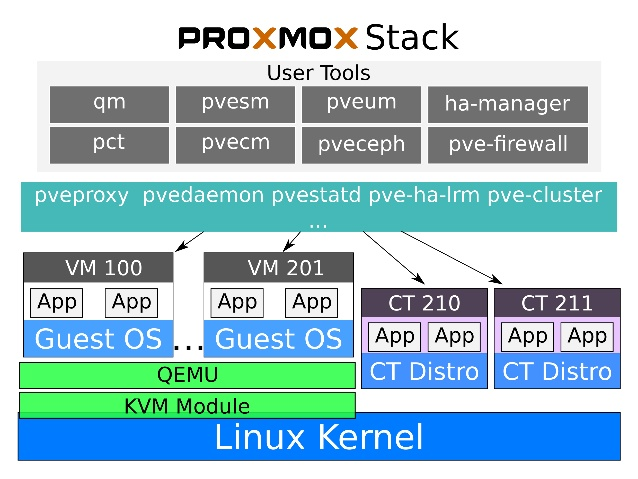
\includegraphics[width=0.6\textwidth]{images/proxmox-stack-example.jpg}

  \end{center}

  \pagebreak

\item
  Setting up a directory to manage users and associated access control policies:
    \\

  We are going to use an LDAP directory as specified in RFC 4510 and following.
  This allows a standardized representation of information (database - LDAP directory) as well as a standard query protocol widely deployed for this database.
  The chosen solution is the OpenLDAP software version 2.4.46, because of its
    maturity and protocol compliance. phpLDAPadmin is the web interface that
    allows the management of user accounts. one of the most important fields is
    sshPublicKey because all the servers are configured to do LDAP queries
    during an SSH connection to list the authorized RSA keys.
    We could have use a PAM setup with libpam-ldap but it seemed easier to specify
    in ssh configuration files an AuthorizedKeyCommand that will reach all the
    RSA public keys on the LDAP server.
  \\ 
  *\url{https://ldap.com/basic-ldap-concepts/}

  \begin{center}

  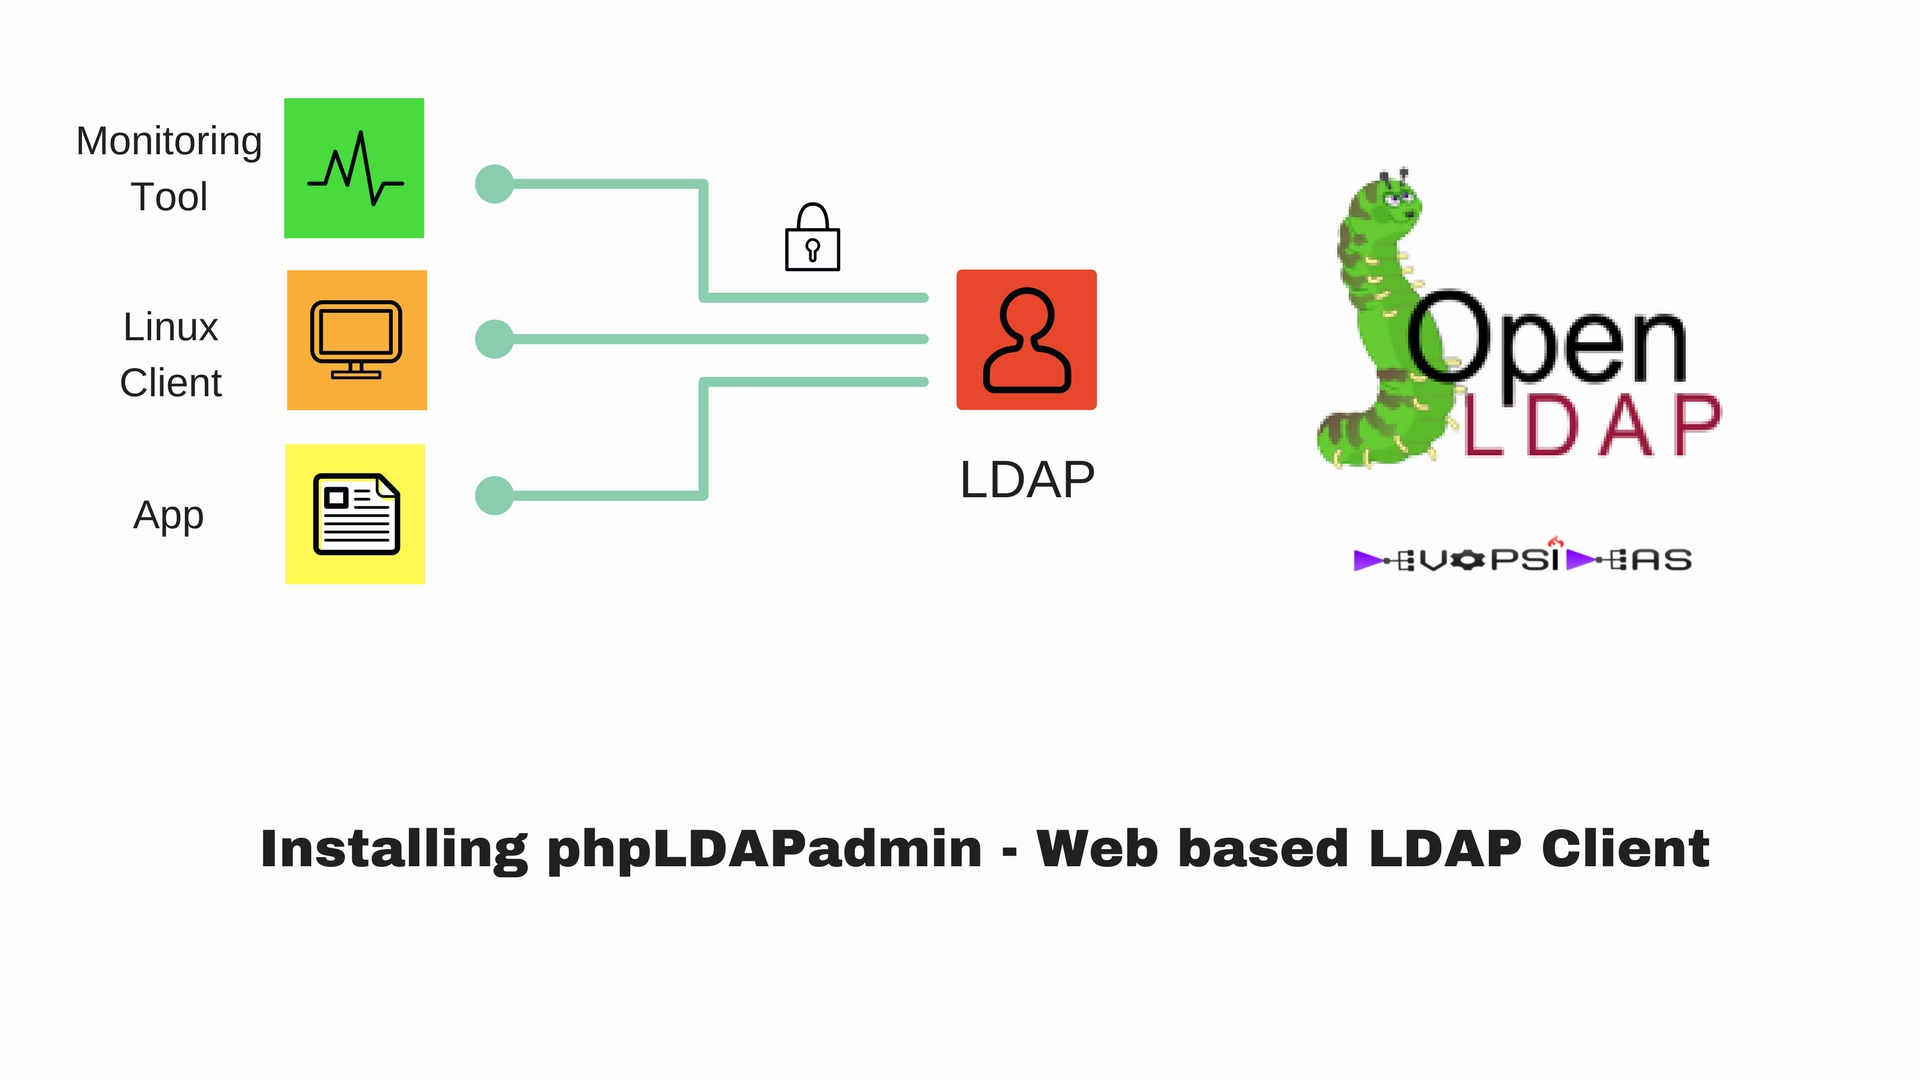
\includegraphics[width=0.75\textwidth]{images/ldap-example.jpg}

  \end{center}

\item
  Use of a tool allowing access to all virtualized machines while using the
    access control protocol cited above: \\

  We are going to use Ansible, an open source software that automates software
  provisioning, configuration management, and application deployment.
  Ansible connects via SSH, remote PowerShell or via other remote APIs.\\ *
  \url{(https://www.ansible.com/)}

  \begin{center}

  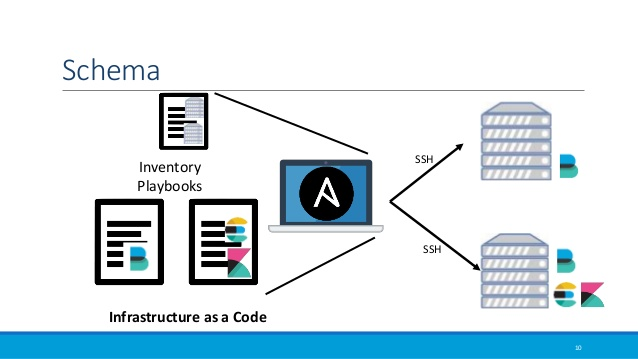
\includegraphics[width=0.75\textwidth]{images/ansible-example.jpg}

  \end{center}

\pagebreak

\item
  Implementation of a list of tools allowing the automated audits added to our
  personal contributions: \\

  For now, Lynis seems to be the best candidate. We will probably combine several tools later.
  Lynis is an extensible security audit tool for computer systems
  running Linux, FreeBSD, macOS, OpenBSD, Solaris, and other
  Unix-derivatives.\\ 
  Lynis scanning is opportunistic, meaning it will only use what it can find, like available tools or libraries. The benefit is that no installation of other tools is needed, so you can keep your systems clean.
By using this scanning method, the tool can run with almost no dependencies. Also, the more it finds, the more extensive the audit will be. In other words: Lynis will always perform scans that are customized to your system and two audits will never be the same!
  \\  * \url{(https://cisofy.com/lynis/)}

  \begin{center}

  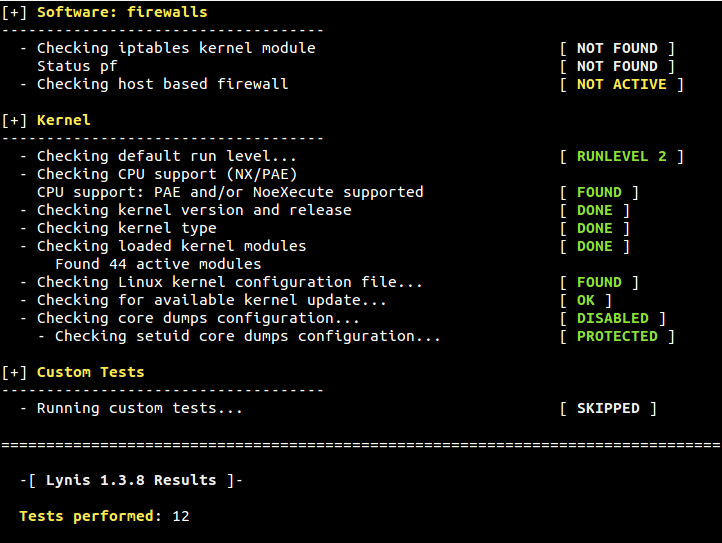
\includegraphics[width=0.95\textwidth]{images/lynis-example.png}

  \end{center}

\pagebreak

\item
  Management of the logs: \\

  ELK is the most famous tool for log processing and analysis, so naturally we will use this tool to generate our logs.
  ELK is the acronym for three open source projects:
  Elasticsearch, Logstash, and Kibana. Elasticsearch is a search and
  analytics engine. Logstash is a server‑side data processing pipeline
  that ingests data from multiple sources simultaneously, transforms it,
  and then sends it to a stash like Elasticsearch. Kibana lets
  users visualize data with charts and graphs in Elasticsearch. The
  Elastic Stack is the next evolution of the ELK Stack.\\ *
  \url{(https://www.elastic.co/fr/elk-stack)}\\
  \begin{center}

  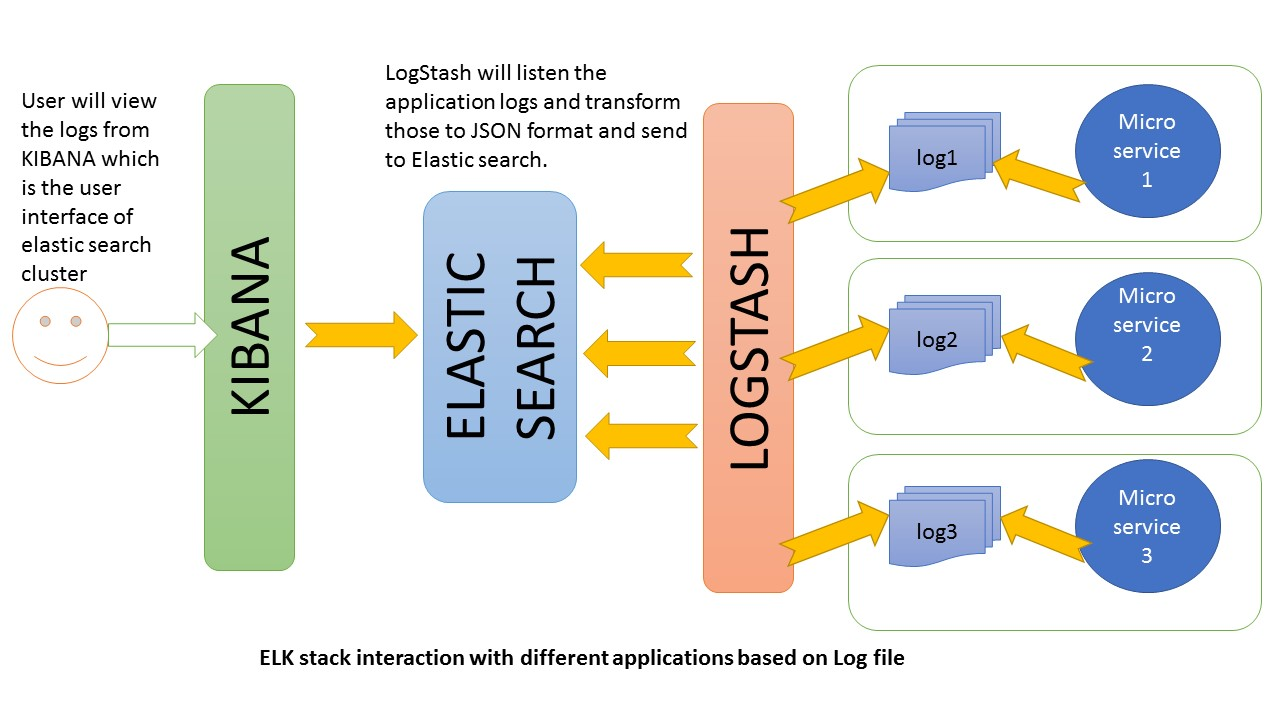
\includegraphics[width=0.75\textwidth]{images/elk-example.jpg}

  \end{center}

\item 
  Web interface development: \\

  The use of a framework associated with a certain number of libraries will
  allow us to obtain a modular and easy to use application.
  Symfony is a PHP framework that we used to manipulate, which is why we chose 
  to use this one. Moreover, we were able to verify that there were many 
  libraries usable by this framework allowing us to interface ELK with our web
  application. \\ *
  \url{(https://pehapkari.cz/blog/2017/10/22/connecting-monolog-with-ELK/)}\\

  \begin{center}

  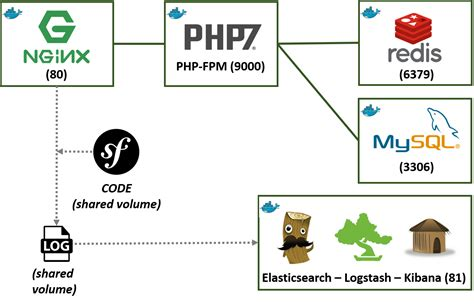
\includegraphics[width=0.65\textwidth]{images/symfony-example.jpg}

  \end{center}


\end{itemize}
\pagebreak

\subsection{Expected results}
\begin{itemize}
\item
  A live demonstration is an option, otherwise, we will record a video 
  of our tool performing an automated audit simulation.
\item
  The presentation of the audit log management and administration platform
  generated by the tool
\item
  To provide a free and open source tool with clear and
  explicit documentation allowing the redeployment of this tool in a virtualized
    environment.
\end{itemize}

We are still looking for other features.

\vspace{1cm}

\subsection{Project Expectations}
The use of English for our project is primodial. Indeed, all the technical
documentation associated with the resources used is in English and we are used
to working with resources in English because they are much more complete. In
addition, the community providing these resources exchanges mainly in English. In order
to offer a tool that is widespread and easy to use, writing the
documentation in English then appears as a better choice. \\
Group size: 3 to 4 students.

\subsubsection{Specific competencies (in addition to PRO4501):}
UNIX-like platforms (Linux, MacOS) and associated tools, including
software development tools (editors, interpretors, etc.). We are working on a
server without a graphical environment so a text editor like VIM should be
optimized as an IDE with some plugins in order to increase our efficiency on the 
server side, on the development and deployment of the tool. 
Coding in JavaScript and / or scripting languages, including referenced 
frameworks for JavaScript development (e.g.~Node.js, Angular.js, etc.)
As Elasticsearch and Kibana are working as APIs, the frontend development part should work
as a REST API too.

\subsubsection{Learning objectives}
Processing of accessible textual data (coherence management, etc.)
, the presentation and analysis of textual data as well as the understanding of cybersecurity
software and integration. \\
Contact: \url{herve.debar@telecom-sudparis.eu} 

%
%% useless according to Hervé Debar
%
%\titlebox{INFORMATION}{Issues related to the project should be addressed exclusively by email.
%It is desirable that interested students contact the project owner. If
%needed, interactions before end of January should occur through
%visio-conference. Project evaluation will be partially linked to the
%achievement of objectives
%}

\pagebreak

\section{Implementation of the project}

\subsection{Little update on tools}

Flask framework imposed after further study of features
necessary techniques for the smooth running of the project. The use of
Proxmoxer (\url{https://github.com/swayf/proxmoxer}) was one of the reasons
main movement to a python framework. \\

Proxmoxer is a wrapper around the Proxmox REST API v2.
It was inspired by slumber, but it dedicated only to Proxmox. It allows to use not only REST API over HTTPS, but the same api over ssh and pvesh utility.
Like Proxmoxia it dynamically creates attributes which responds to the attributes you've attempted to reach.
\\

\lstinputlisting[language=Python]{scripts/proxmoxer.py}

\subsection{Network Architecture}

\vspace{2cm}

\begin{center}
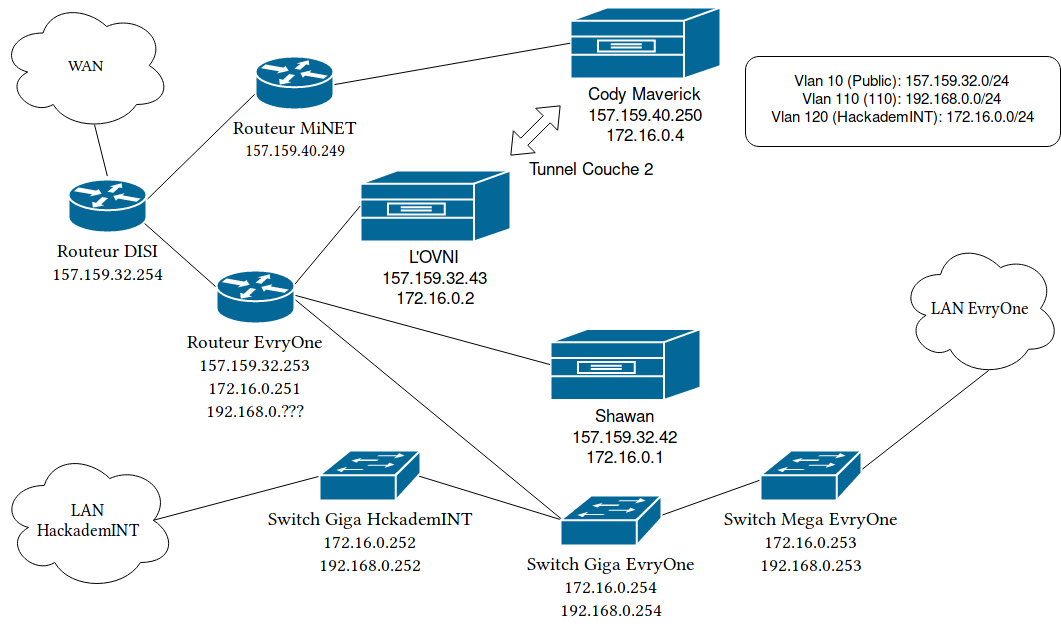
\includegraphics[width=0.95\textwidth]{images/reseau.png}
\end{center}

\pagebreak

\subsection{Application Architecture}

Here is the detail of the architecture as currently designed for this project:
\begin{itemize}
\item
  Several physical servers (whose names are "Cody-Maverick", "L'OVNI" and
  "Shawan") have been clustered on which are deployed the Proxmox hypervisor.
\item
  Flask application dialog with this hypervisor through its API, we
  so use proxmoxer as a wrapper to interface with
  it.
\item
  It is possible to access containers and virtual machines through
  pct (Tool to manage Linux Container (LXC) on Proxmox VE) and
  qmu (Qemu / KVM Virtual Machine Manager).
\item
  To connect to different machines in the infrastructure, the application
  knows the IP addresses of the different machines thanks to the API of
  the hypervisor and RSA private keys must be filled in by the administrator
  system within the application to allow connection to
  different machines.
\item
  By using the SSH network protocol, the Ansible tool helps with the execution of
  Lynis security audit tool on the different in order to get a
  log file which will then parser and embed in the ELK stack, itself
  interfaced with the application. We thus obtain a complete report of the
  security of every machine within the application
\item
  User management of the application is performed at a base level
  postgresql data that the application accesses via the SQlachemy ORM.
\end{itemize}


\vspace{1cm}
\begin{center}
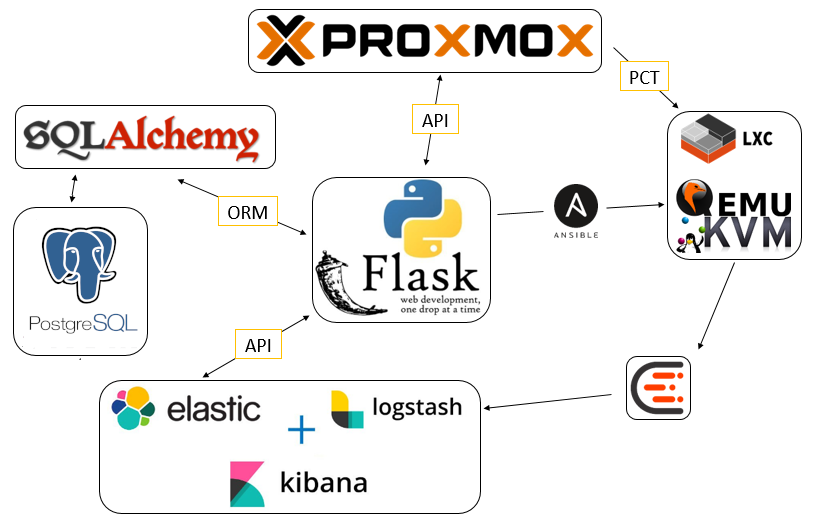
\includegraphics[width=0.90\textwidth]{images/schema.png}
\end{center}

\pagebreak

\subsection{Scoring and standardization}

The Common Vulnerability Scoring System (CVSS) is a free and open industry standard for assessing the severity of computer system security vulnerabilities. CVSS attempts to assign severity scores to vulnerabilities, allowing responders to prioritize responses and resources according to threat. Scores are calculated based on a formula that depends on several metrics that approximate ease of exploit and the impact of exploit. Scores range from 0 to 10, with 10 being the most severe. While many utilize only the CVSS Base score for determining severity, temporal and environmental scores also exist, to factor in availability of mitigations and how widespread vulnerable systems are within an organization, respectively.
\\ 
With Lynis, many tests are part of common security guidelines and standards,
with on top additional security tests. After the scan a report will be displayed
with all discovered findings. Our application will map these vulnerabilities with a CVSS Base, Temporal and Enrironmental Score 

\vspace{1cm}
\begin{center}
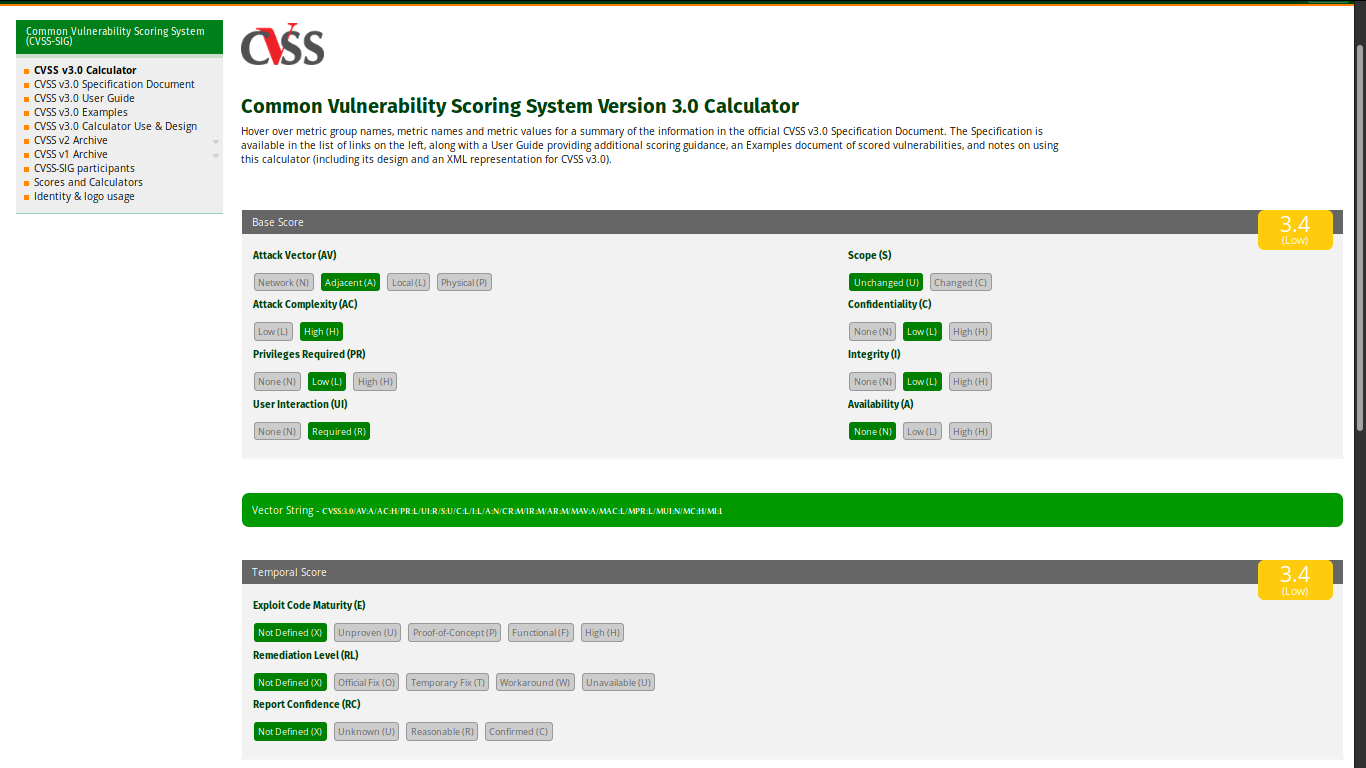
\includegraphics[width=0.98\textwidth]{images/cvss.png}
\end{center}
\pagebreak

\subsection{Results}

\vspace{1cm}
\begin{center}
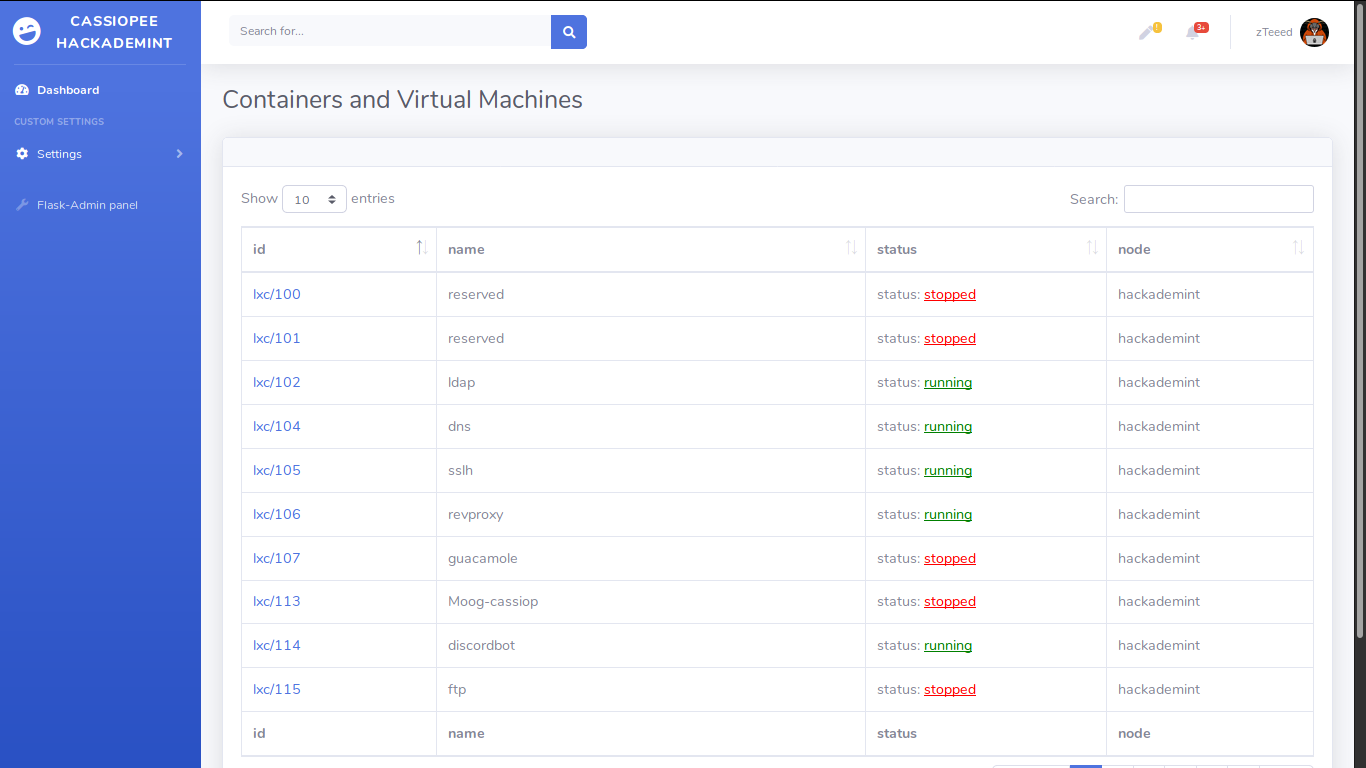
\includegraphics[width=0.98\textwidth]{images/flask-application-1.png}
\end{center}
\vspace{1cm}
\begin{center}
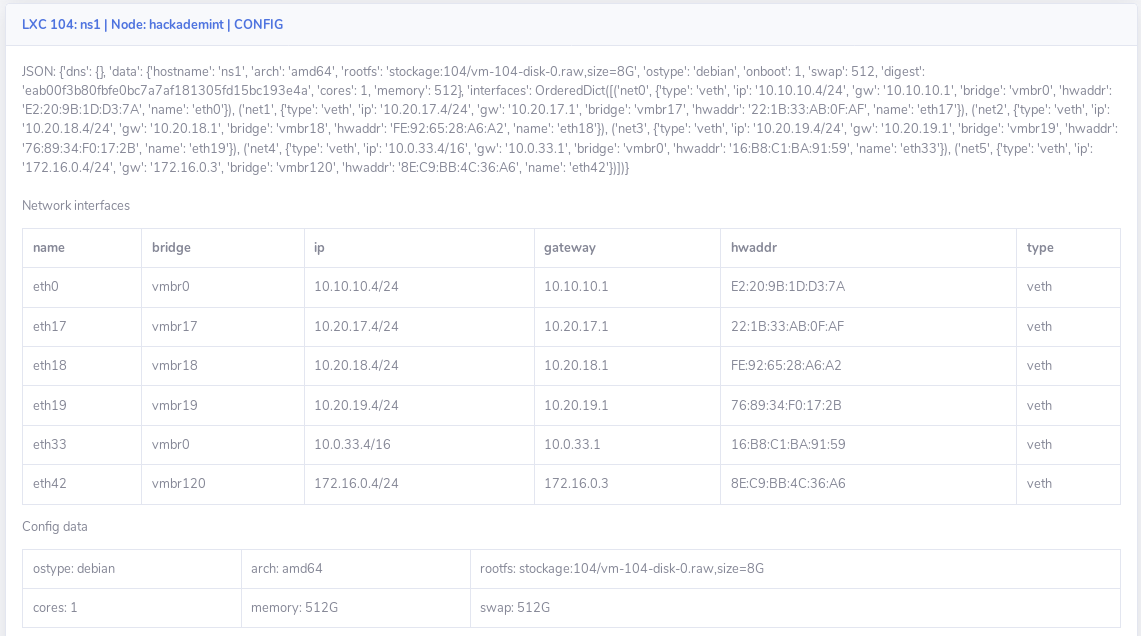
\includegraphics[width=0.98\textwidth]{images/flask-application-2.png}
\end{center}
\vspace{1cm}
\begin{center}
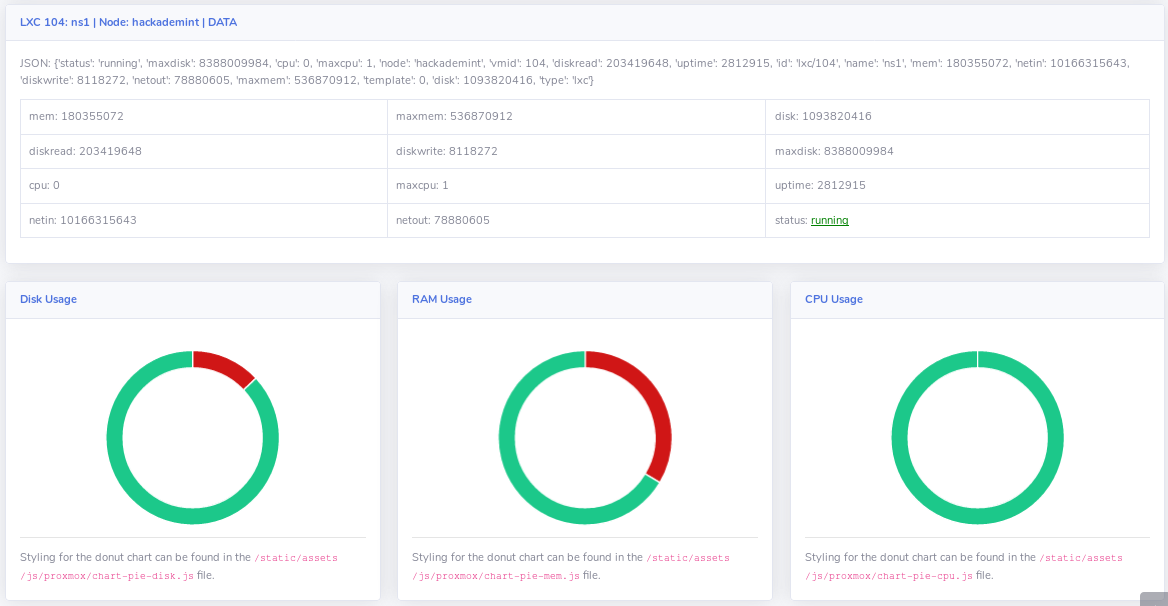
\includegraphics[width=0.98\textwidth]{images/flask-application-3.png}
\end{center}

\end{document}
